% Tutorial 03

\subsection{Tutorial 3: Using HREMD and distance-field}
Another way to calculate the binding free energy of a ligand to a protein is to pull the ligand out of the active site. 
There are several methods available to perform such calculations, however, most of them require the \textit{a priori} knowledge of the dissociation path. 
Even if the dissociation path is determined during the simulation, it is often assumed that it is linear, or that only a single dissocation path exists. 
For an accurate estimate of the binding free energy the simulations should be performed such that the binding and unbinding of the ligand can be sampled reversibly.
In this tutorial we will use the distance-field (DF) distance as the reaction coordinate and combine this with Hamiltonian-replica-exchange molecular dynamics (HREMD) simulations~\cite{deRuiter_2013}.
The advantage of the DF distance is that we will be able to pull the ligand back into the active site, even if it moved to the other side of the protein. 
The HREMD simulations allow for multiple paths to be sampled reversibly~\cite{Nagy_2017}.

\subsubsection{Preparations}
As in the tutorial above, we will use the PLA$_2$ - ASA complex as a test system. 
The preparation of the topology, coordinates, the energy minimization and the equilibration of the system are very similar to the tutorial above. 
The only difference is that we will use a larger cubic box to allow the ligand to move freely in the solvent. 
The final equilibrated structure can be found in the directory \texttt{eq} with the name \texttt{eq\_PLA2\_ASA\_Ca\_2Na\_7.cnf}.

\subsubsection{Slow-growth}
In order to get some initial coordinates for each of the replicas of the HREMD simulations, we will perform a short slowgrowth simulation where the ligand is pulled out of the active site in a non-equilibrium manner. 
The exact pulling speed and force constant are not relevant in this case as we are not trying to calculate the binding free energy from the slow-growth simulations. 
It is, however, important that the structure of the protein does not get disrupted during this initial simulation. 
The slow-growth simulation is started from the final configuration of the equilibration. 
Go to the directory \texttt{slowgrowth} and have a look at the \texttt{PERTURBATION} block in the input file \texttt{slowgrowth.imd}. 
\begin{lstlisting}
PERTURBATION
#     NTG   NRDGL    RLAM   DLAMT
        1       0     0.0   0.001
#  ALPHLJ   ALPHC    NLAM  NSCALE
      0.0     0.0       1       0
END
\end{lstlisting}
With \texttt{NTG} set to \texttt{1}, you specify that a free energy calculation will be performed. 
The starting $\lambda$ point \texttt{RLAM} is set to \texttt{0}. With each timestep during the simulation, $\lambda$ will be increased. The rate of increase in ps$^{-1}$ is set to \texttt{DLAMT = 0.001}. 
Together with \texttt{NSTLIM = 500000} (from the \texttt{STEP} block) and an integration time step of 0.002~ps this results in a simulation of 1ns where $\lambda$ is continuously changed from 0 to 1. 
\texttt{ALPHLJ} and \texttt{ALPHC} are the softness parameters of the Lennard-Jones and Coulombic interactions, respectively. 
These are set to 0 here, because we are not changing any nonbonded interactions, only distance restraints. 
In addition to that, we have to specify which kind of restraints will be used. In this case we will use distance-field distance restraints:
\begin{lstlisting}
DISTANCEFIELD
# NTDFR
      1
#  GRID PROTEINOFFSET PROTEINCUTOFF PROTECT
    0.2       15          0.2             0
# UPDATE  SMOOTH   RL   NTWDF     PRINTGRID
    100        1  1.0    1000             0
END
\end{lstlisting}
With \texttt{NTDFR} set to \texttt{1}, we turn on distance-field (DF) restraining during the simulation. Typically the grid size (\texttt{GRID}) for the DF calculation is set to 0.2~nm. 
\texttt{PROTEINOFFSET} is the penalty which is added to the DF distance if the path crosses the host. 
This value has to be large enough, such that paths through the protein always result in larger DF distances than around the protein. 
If the length of paths around the protein is larger than the value of \texttt{PROTEINOFFSET}, the paths that go through the protein may become competitive and forces will point into the protein, 
rather than along the surface. Setting very large values of \texttt{PROTEINOFFSET} however, may lead to large forces at the surface of the protein, especially if the \texttt{SMOOTH} option is not used (see below).
Here we have chosen \texttt{PROTEINOFFSET = 15}~nm. 
\texttt{PROTEINCUTOFF = 0.2} determines that any grid point which is within 0.2 nm of a protein atom will be flagged as protein. 
In cases where the binding site is quite small, it can happen that the zero distance point is often flagged as protein, in these cases it might be necessary to use \texttt{PROTECT > 0}. 
This is the radius around the zero-distance point in which a grid point will not be flagged as protein. For our simulation, we will leave this value at \texttt{0}. 

In order to speed up the simulation, the grid is calculated only every \texttt{UPDATE = 100} steps. 
The \texttt{SMOOTH} parameter is used to prevent very large forces acting at the surface of the protein due to the large penalties. 
With each smoothening step the non-protein grid points are identified which have a direct neighbouring grid point flagged as protein. 
These are on the edge of the protein and we will recalculate their DF distance but now without the protein penalty. 
This removes the large forces pointing away from the protein, but because the smoothening steps are performed after the updating step, they do not influence the optimal route. 
We will set the number of smoothening rounds to \texttt{1}. Forces change linearly for distances larger than 1 nm as set by \texttt{RL}. 
We will write DF distances and forces to an external file (special trajectory file, *.trs) every \texttt{NTWDF = 1000} steps. We will not print the grid to the final configuration, so we use \texttt{PRINTGRID=0}. 
The definition of the distance restraint that will be modified during the slow-growth simulation, is specified in the distance restraint specification file \texttt{disres.dat}. 
There are two blocks in this file. 
The first one, \texttt{DISTANCERESSPEC} specifies the distance restraints between the Ca$^{2+}$ ion and its surrounding residues, which prevents the Ca$^{2+}$ from drifting away. 
The second block \texttt{PERTDFRESSPEC} specifies the perturbed distance-field restraints. 
\begin{lstlisting}
PERTDFRESSPEC
# DISH  DISC
  0.1   0.153
# PROTEINATOMS  A_R0  K_A  B_R0  K_B  M  N
          1190   0.0  500   5.0  500  0  0
#  TYPE_I  NUM_I ATOM_I[0] .. ATOM_I[NUM_I]
       -1      7    16 190 249 312 486 632 1208
#  TYPE_J  NUM_J ATOM_J[0] .. ATOM_J[NUM_J]
       -1      2  1194 1203
END
\end{lstlisting}
\texttt{DISH = 0.1}~nm specifies the carbon - hydrogen distance and \texttt{DISC = 0.153}~nm specifies the carbon-carbon distance. % in nm. 
These are used to compute the position of some types of pseudo or virtual atoms, respectively, from the positions of explicitly represented atoms.
\texttt{PROTEINATOMS} specifies the last atom number of the protein which will be used to flag protein atoms. 
\texttt{A\_R0} and \texttt{B\_R0} are the restraining distances in nm at \texttt{$\lambda$ = 0} and \texttt{$\lambda$ = 1}, respectively. 
We will use a force constant of 500 kJ mol$^{-1}$ nm$^{-2}$ which remains the same upon changing $\lambda$ (\texttt{K\_A = K\_B = 500}). 
We will not use hidden distance restraints, so \texttt{M = N = 0}. 

The distance between pseudo atom \texttt{i} and pseudo atom \texttt{j} will be restrained, where pseudo atom \texttt{i} is defined as the center of geometry of 7 atoms (\texttt{NUM\_I = 7}) with atom numbers 16, 190, 249, 312, 486, 632 and 1208. 
These atom numbers correspond to the $C_{\alpha}$ atoms of residues L2, W18, A22, C28, D48, Y63 (residue numbers according to the topology) and the calcium ion. 
Pseudo atom \texttt{j} is the center of geometry of atoms C2 and C7 (topology names) of the aspirin ligand. 
All input files are now prepared and we can generate the run file with:
\begin{lstlisting}
$ mk_script @f mk_script.arg
\end{lstlisting}
Make sure the generated \texttt{slowgrowth\_PLA2\_ASA\_1.run} file is ready to be submitted to a cluster. 
After running the slow-growth simulation, we can analyze the system by using \texttt{trs\_ana}. 
We will use this program to read out the DF distances and forces from the special trajectory, \texttt{*.trs}, file. An example of the argument file is prepared in \texttt{trs\_ana.arg}. 
You can run the program with 
\begin{lstlisting}
$ trs_ana @f trs_ana.arg
\end{lstlisting}
The DF distance as a function of time is written out to the file \texttt{df\_dist.dat}. Have a look at the file with e.g. Xmgrace and make sure no sudden jumps are present. 
We also need to make sure that the protein was not disrupted during the pulling process. For this, calculate the root-mean-square deviation (RMSD) as a function of time with
\begin{lstlisting}
$ rmsd @f rmsd_bb.arg > rmsd_bb.dat
$ rmsd @f rmsd_all.arg > rmsd_all.dat
\end{lstlisting}
Have a look at the RMSD of the backbone atoms (\texttt{rmsd\_bb.dat}) as well as for all protein atoms (\texttt{rmsd\_all.dat}). 
When both the \texttt{df\_dist.dat} and the RMSD plots look normal, we can continue to prepare the starting structures for the replica-exchange simulations. 
If not, the slow-growth simulation should be performed again with some variables modified.
For example, you can decrease \texttt{DLAMT} (and increase \texttt{NSTLIM} accordingly) in order to pull slower. 
Changing the force constant of the DF restraints (\texttt{K\_A} and \texttt{K\_B} in the \texttt{PERTDFRESSPEC} block) or choosing different atoms to apply the DF restraints to can also help to avoid any disruption of the protein.

\subsubsection{Hamiltonian-replica-exchange simulations}
One of the first choices that we have to make when starting a HREMD simulation, is how many replicas will be used. 
For performance issues it is best to keep the number of replicas equal to the number of CPUs available (preferably on a single computational node). 
In the prepared example, we used 24 replicas. Have a look at the prepared input file for the replica-exchange simulation (\texttt{HREMD.imd} in the directory \texttt{HREMD}). 
You will find that the \texttt{PERTURBATION} block is still present, but with \texttt{DLAMT} now set to \texttt{0}. 
This means we are still calculating free energies, but we are no longer changing the $\lambda$ parameter during a single simulation. 
The \texttt{DISTANCEFIELD} block is pretty much unchanged, apart from \texttt{NTWDF} because we will write out the DF data more often. You will also find an additional block:
\begin{lstlisting}
REPLICA
# NRET
  1
# RET(1..NRET)
  298.0
# LRESCALE
  0
# NRELAM
  24
# RELAM(1..NRELAM)
 0.0000 0.0435 0.0870 0.1304 0.1739 0.2174 0.2609 0.3043 0.3478 0.3913 0.4348 0.4783 0.5217 0.5652 0.6087 0.6522 0.6957 0.7391 0.7826 0.8261 0.8696 0.9130 0.9565 1.0000
# RETS(1..NRELAM)
 0.002  0.002  0.002  0.002  0.002  0.002  0.002  0.002  0.002  0.002  0.002  0.002  0.002  0.002  0.002  0.002  0.002  0.002  0.002  0.002  0.002  0.002  0.002  0.002
# NERTRIAL
  100
# NREQUIL
  0
# CONT
  1
END
\end{lstlisting}
Because we will perform Hamiltonian-replica-exchange and not temperature replica exchange, the number of replica exchange temperatures are set to \texttt{NRET=1}. 
We thus also only have one \texttt{RET} value which is the temperature of each replica, in this case equal to 298~K. 
We do not need to scale temperatures after exchange trials, so \texttt{LRESCALE=0}. \texttt{NRELAM} is the number of replica-exchange lambda values, which is set to 24 here. 
For each of the replicas you have to specify at which $\lambda$ value it should be simulated. These values are given at \texttt{RELAM}. 
We do not know the optimal spread of the $\lambda$ values of the replicas before actually running the simulations, so as an initial guess we just spread them evenly between $\lambda$ = 0 and 1. 
We will keep the standard timestep of 0.002 ps for each $\lambda$-replica, as given by \texttt{RETS}. 
In order to keep the simulation time per run short, we set the number of exchange trials per run to \texttt{NERTRIAL=100}. 
Prolonging the simulations can then be done by performing multiple runs sequentially. 
\texttt{NREQUIL} sets the number of exchange periods for equilibration, during which no switches between the replicas are allowed. 
This would be especially beneficial if you start the HREMD simulations from a single configuration and you need time to equilibrate. 
Since we start from multiple configurations which are close to their respective $\lambda$ values, we will set this to 0. 
\texttt{CONT=1}, as we start from multiple configuration files, instead from a single configuration.
The next step will be to select the appropriate configurations from the slow-growth simulation as initial configurations for each of the replicas.

The script \texttt{write\_start\_files.py} in the directory \texttt{starting\_coordinates} will help with this. 
The program will find the $\lambda$ values of the replicas, look for the DF restraint in the PERTDFRESSPEC block in the distance restraints file and determine the restraining distances for each of the replicas from this information.
It will then search for the frame in the slow-growth simulation which has a DF distance which is closest to the restraining distance of this replica.
This frame will be written to a separate file for each of the replicas, named \texttt{start\_\{X\}.cnf}, where \texttt{X} will be the replica number. 
An example argument file is provided which lists the topology of the system, the DF distances over time of the slow-growth simulation (\texttt{df\_dist.dat}), the coordinate trajectory from the slow-growth simulation, the HREMD input file and the distance restraint specification file as will be used for the HREMD simulation. To run the script:
\begin{lstlisting}
$ ./write_start_files.py @write_start_files.arg 
\end{lstlisting}
The starting coordinates for the HREMD simulation are now available and we can prepare the run files with \texttt{mk\_script}:
\begin{lstlisting}
$ mk_script @f mk_script.arg
\end{lstlisting}
The HREMD simulations are split into quite a few runs, in order to prevent an extremely long single simulation. 
Go to the first directory, \texttt{run1} and submit \texttt{HREMD\_1.run} to a computer cluster, preferable with the same number of CPUs as we have replicas, which would be 24 in the prepared example. 

\subsubsection{Analysis of HREMD}
All analyses for HREMD simulations will be performed in the subfolder \texttt{analysis}. 
In order to make sure the choice of replicas is appropriate, we will analyze whether there were sufficient switches between the replicas. This can be done already after only a few runs have finished. 
The switching information of the replicas is written out to the \texttt{replica.dat} file for each of the runs separately. 
You can combine them into a single file by using the provided script:
\begin{lstlisting}
$ ./gather_replica_data.sh [nr_runs] [nr_trials]
\end{lstlisting}
Here, you need to replace [nr\_runs] with the number of runs which have been performed already and [nr\_trials] with the number of exchange trials per run, which was set to 100 in the example files.
This script results in the file \texttt{replica\_all.dat}. The switches of the replicas can now be visualized by running
\begin{lstlisting}
$ ./rep_ana_mpi.py replica_all.dat
\end{lstlisting}
The resulting \texttt{rep\_change.out} file can be opened with \linebreak Xmgrace. An example of such file is shown in  Figure~\ref{rep_change}.

\begin{figure}[H]
\centering
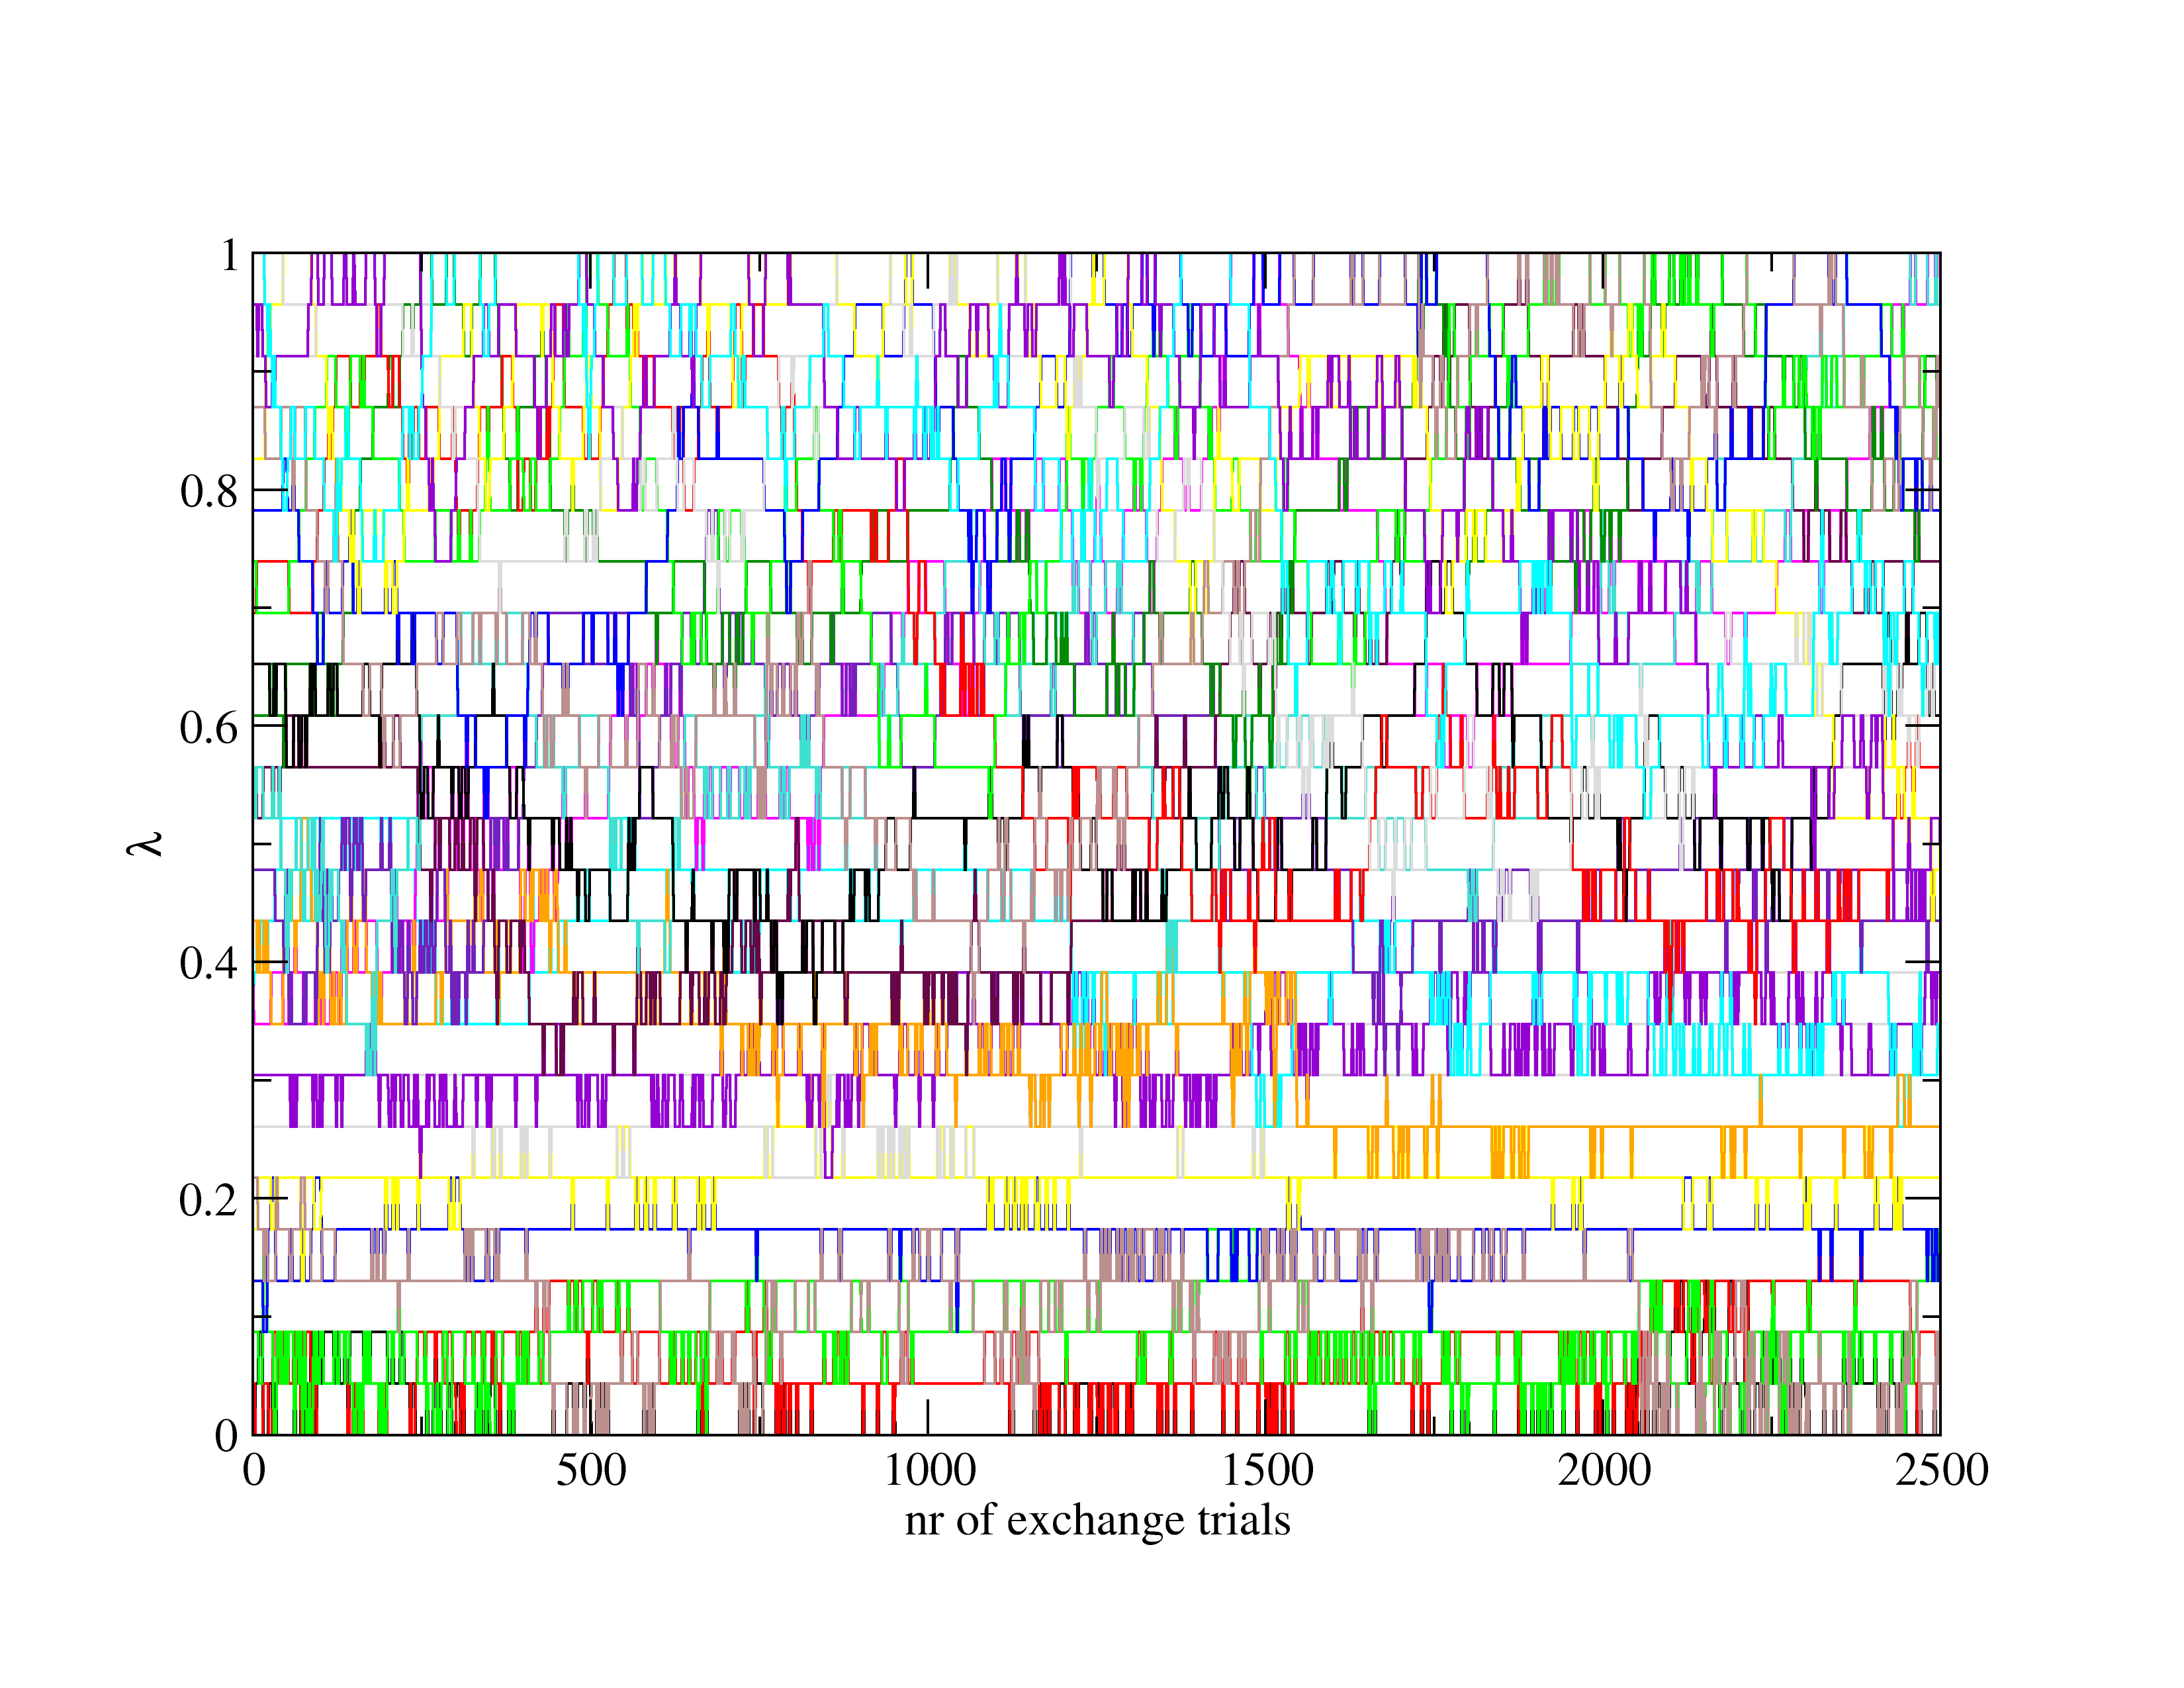
\includegraphics[scale=.3]{../06_tutorial_03/figures/rep_change}
\caption{Replica exchanges during time. Different colors represent different replicas.}
\label{rep_change}
\end{figure}

In case there is a pair of $\lambda$ points for which not enough switches are occurring, you have two options to resolve this. 
You can either insert another $\lambda$ point or make the difference between the $\lambda$ points smaller. 
The former option is maybe quicker to set up, but requires longer simulation time because of the additional replica. 
The latter option does not require more replicas, but it is not guaranteed that your small change improves the switching probabilities and that you do not introduce another region of low switching probability due to the change.
Of course you can also use more elaborate methods to optimize the $\lambda$-spacing \cite{Hritz_2007}.

If you are happy with the switching probabilities, you can start preparing for the calculation of the Free Energy Curve (FEC).
First, we have to write out the measured DF distances for each of the replicas. Then we calculate the distributions of these and on this data we can perform the weighted histogram analysis method (WHAM) which will result in the FEC.
We will again use the program \texttt{trs\_ana} to extract the DF distance from the special trajectories (\texttt{*trs.gz}). 
A small script is provided which runs this program for each of the replicas, thereby collecting data from each of the runs.

\begin{lstlisting}
$ ./do_all_trs_ana.sh [nr_runs] [nr_replicas]
\end{lstlisting}
This will generate a subdirectory called \texttt{df\_dist} which then contains \texttt{df\_dist\_X.dat} files for each replica X. 
From these distance files, we will first generate the distributions, which can then be used to determine the FEC by applying WHAM. 
The program \texttt{tcf} can generate distributions for each of the \texttt{df\_dist} files. 
We will set the boundaries to 0 and 5 nm (the same range as the restraining distances) and use 200 bins. 
Especially the boundaries should be adapted when working on different systems. 
Again, a small script is prepared which will perform the program \texttt{tcf} on each of the replicas:

\begin{lstlisting}
$ ./do_tcf.sh [nr_replicas]
\end{lstlisting}
One should always check whether the distributions at adjacent $\lambda$-values are sufficiently overlapping and whether the individual distributions are sufficiently sampled.
We can then determine the FEC $F(r)$ by using the WHAM program. 
Note that the FEC contains the Jacobian contribution, whereas a PMF does not \cite{Trzesniak_2007}. 
As input parameters, the WHAM program needs the temperature of the simulation, the restraining distance for each replica and the force constant of the restraints. 
All this information is read from the \texttt{HREMD.imd} and \texttt{disres.dat} files as specified in the \texttt{do\_wham.sh} file:
\begin{lstlisting}
$ ./do_wham.sh
\end{lstlisting}
This script also moves the final FEC on the y-axis such that its minimum is placed at 0 kJ/mol.
The file \texttt{wham\_FEC\_200bins\_5000iter\_min0.dat} now contains the final FEC, which is shown in Fig.~\ref{FEC}. As you can see, the curve is not completely flat at larger distances, but is rather noisy. Ideally, you would have to change the spacing of the replicas, add more replicas in the unbound range, or lower the maximum distance which you restrain such that the replicas are placed more densely in the unbound range. 
However, we can still see where the plateau of the unbound range is, so we will go ahead with the calculation of the binding free energy.

\begin{figure}[H]
\centering
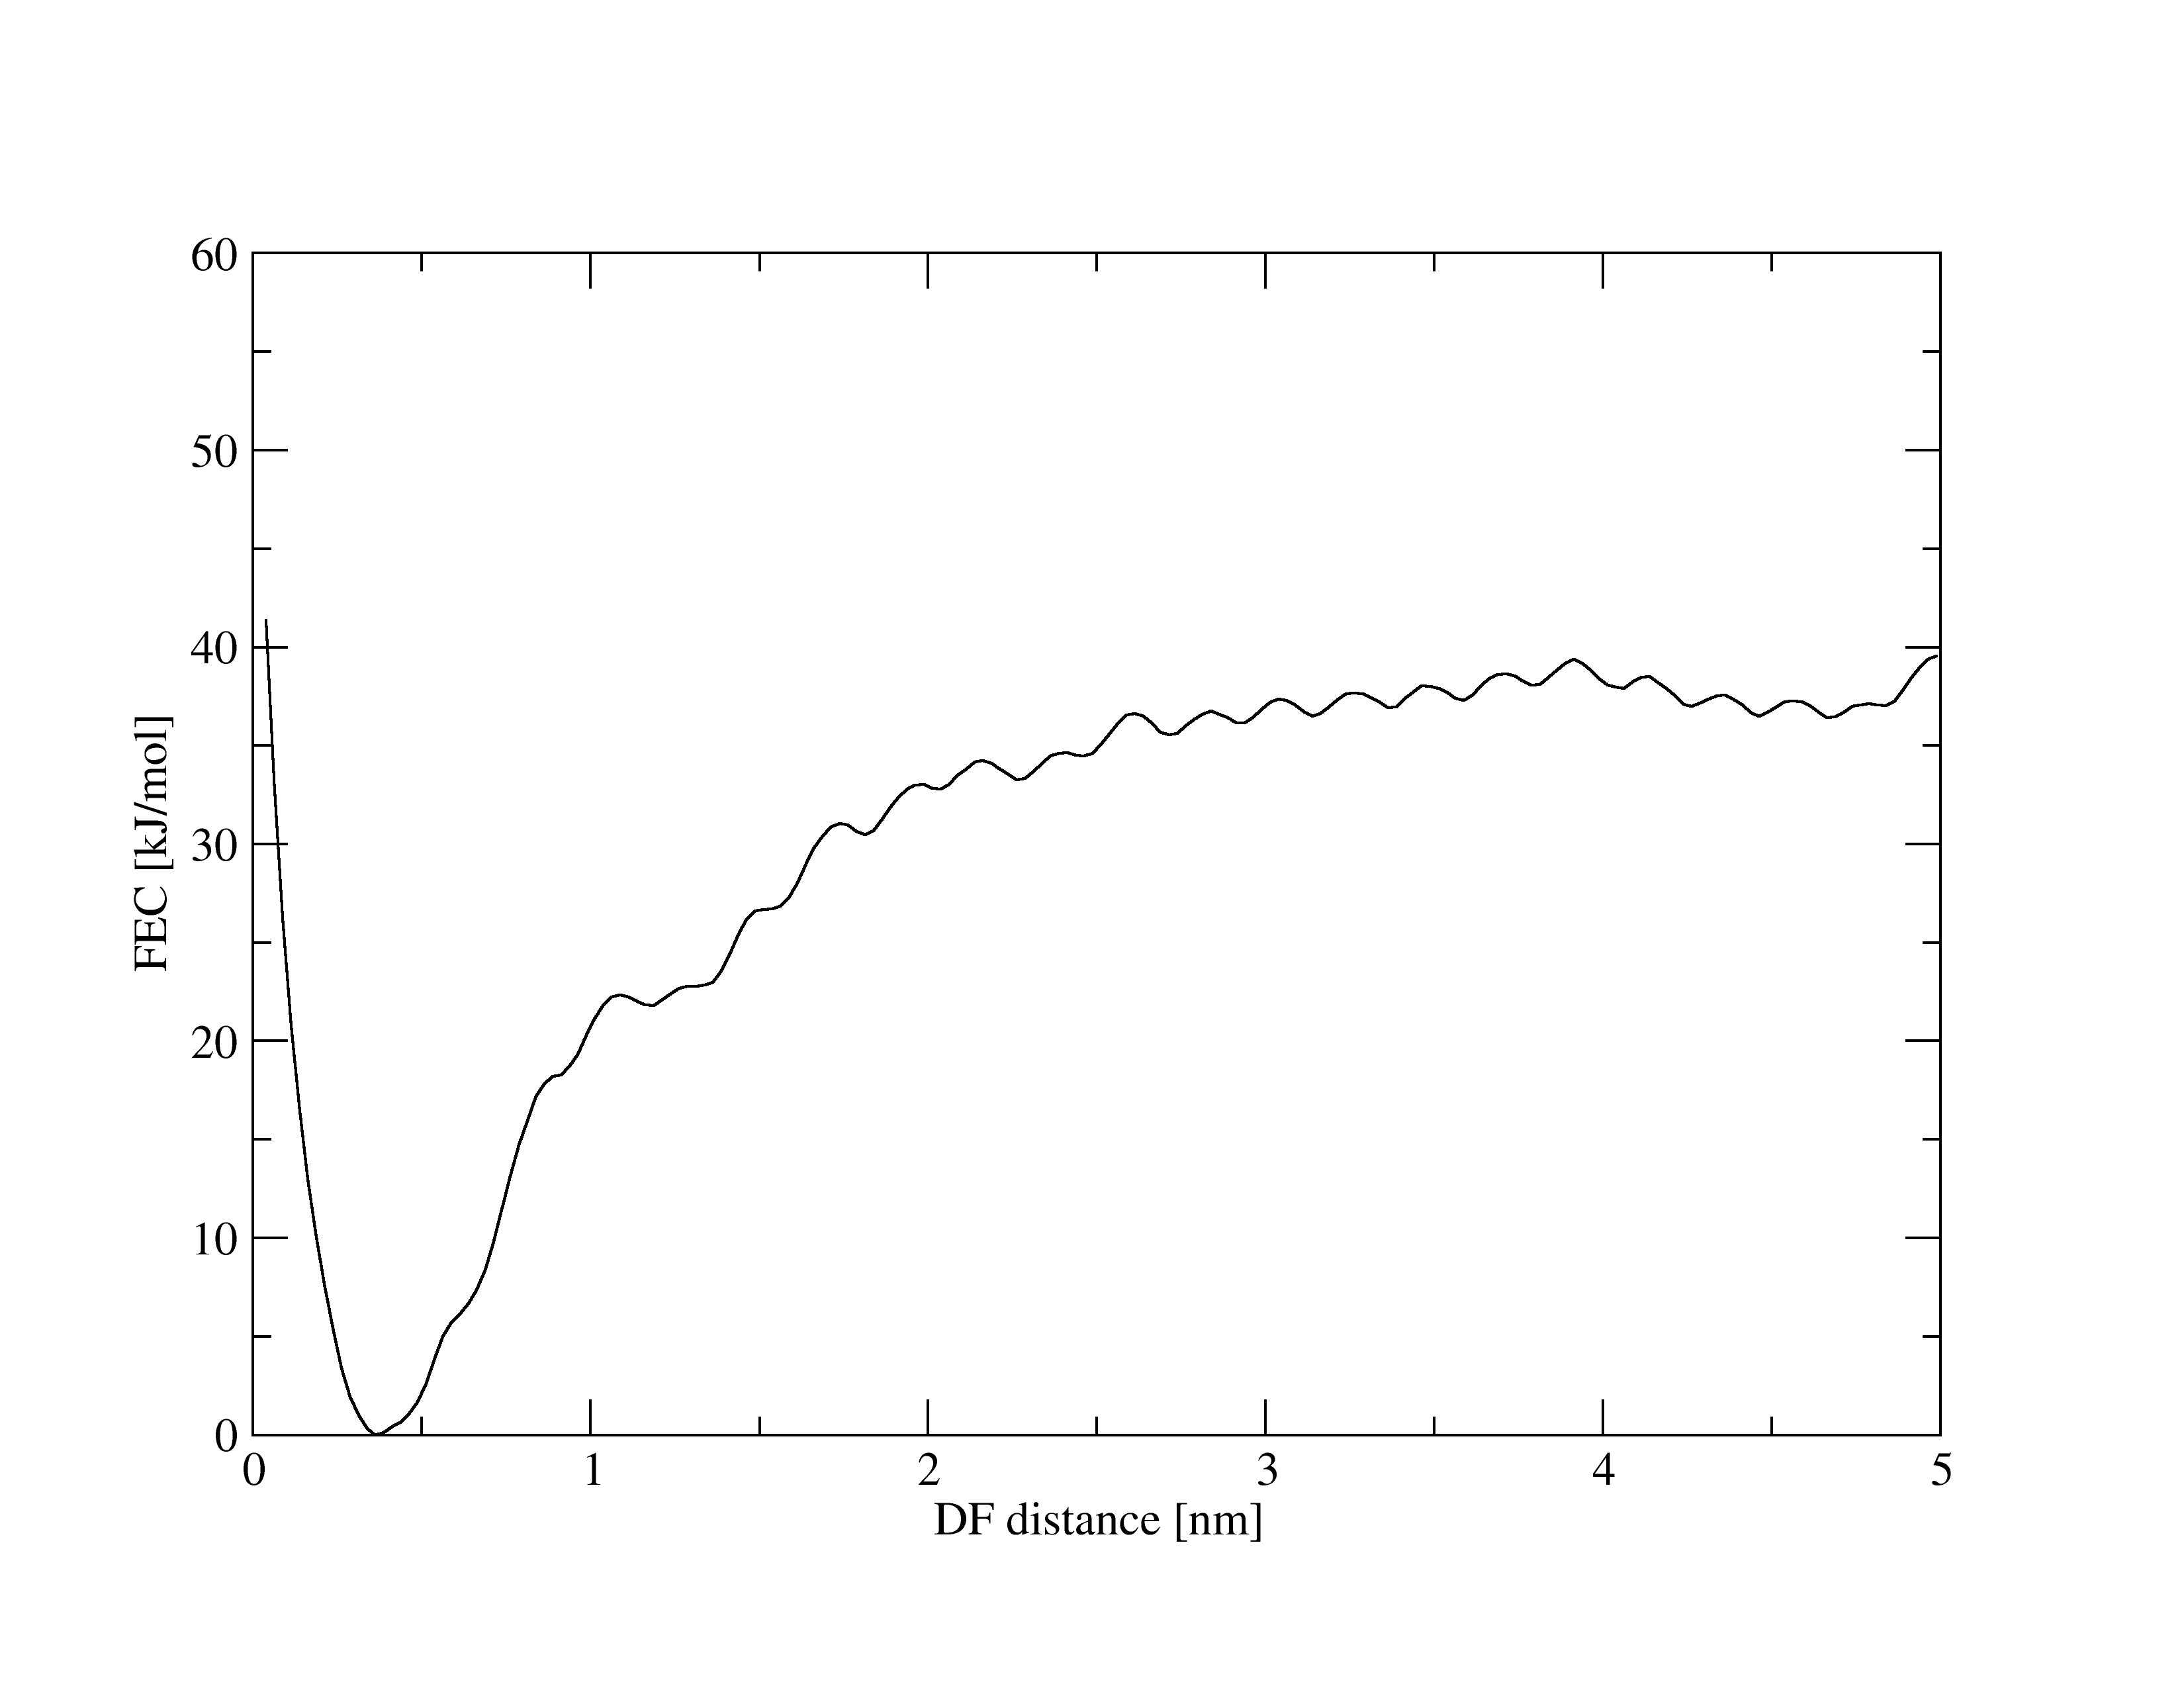
\includegraphics[scale=.3]{../06_tutorial_03/figures/FEC}
\caption{Free Energy Curve (FEC) along the DF distance as obtained from HREMD simulations, for the PLA2-ASA system.}
\label{FEC}
\end{figure}

\subsubsection{Calculation of binding free energy}

To derive the binding free energy from the FEC in Fig.~\ref{FEC} we cannot simply take the value of $\Delta G$ at the plateau around the unbound state. We will need to integrate the bound and unbound ranges of the FEC and we will need to include the standard state correction of 
\begin{equation}
\Delta G_{\text{std}} = -k_{\text{B}}T \ln \left (\frac{V_{\text{u}}}{V^{\circ}} \right )
\end{equation}
Here, $V^{\circ}$ is the standard state volume of 1.661 nm$^3$ and $V_{\text{u}}$ is the unbound volume which is sampled by the ligand in the unbound range.
This range is defined by the plateau observed in the FEC curve.  

In order to determine $V_{\text{u}}$ we need to select the configurations of the trajectory which contributed to the plateau range of the FEC. 
In this example, the plateau can be observed between 3 and 5 nm. 
The script \texttt{select\_frames\_unbound\_region.sh} (which you can find in the subdirectory \texttt{unboundVolume}) will select the appropriate frames by reading in the \texttt{df\_dist\_X.dat} files which were generated using \texttt{do\_all\_trs\_ana.sh}.
Since the DF distances are written out every 50 steps (\texttt{NTWDF=50}) and the coordinates only every 1000 steps (\texttt{NTWE=1000}), the script filters the \texttt{df} distance file such that it matches the timesteps of the coordinate trajectory. 
In order to run the program, specify the number of replicas, the number of runs and the boundaries of the unbound range:
\begin{lstlisting}
$ ./select_frames_unbound_region.sh 24 [nr_runs] 3.0 5.0
\end{lstlisting} 
%In this case the energy trajectory was written out every \texttt{NTWE=50} steps and the coordinates only every \texttt{NTWX=1000}, so we take only every 20th frame of the energy trajectory into account.
%The small script \texttt{do\_ene\_ana.sh} runs the program \texttt{ene\_ana} and filters the result such that it matches the timesteps of the coordinate trajectory.
%In order to run the program, specify the replicas which mark the unbound region, as well as the number of runs;
%\begin{lstlisting}
%$ ./do_ene_ana.sh 15 24 [nr_runs]
%\end{lstlisting} 
%Another program is then used to select the frames which have zero interaction energy and to write out the corresponding snapshots of the coordinate trajectory;
%\begin{lstlisting}
%$ ./select_frames_0kJ.sh 15 24 [nr_runs]
%\end{lstlisting}
%The results are written to different directories for each of the replicas.
A list of the selected configurations (\texttt{list\_frames\_unbound\_\\region.txt}) as well as the trajectory with only these configurations (\texttt{unbound\_region\_frames.trj}) are written to separate directories for each of the replicas.
%For each of the replicas in the unbound region, we will then determine how much volume was sampled in these selected frames.
We will now combine all the configurations from the unbound range and determine how much volume was sampled by the ligand by using the program \texttt{iondens}.
\texttt{iondens} calculates the average density of ions (ligand in our case) from a trajectory file.
For the example, here you can start it with
\begin{lstlisting}
$ ./do_iondens.sh 
\end{lstlisting}
where we use the final configuration from the equilibration run as a reference configuration. 
Some parameters in \texttt{do\_iondens.sh} have been set as appropriate for the current system.
For example, the particle that we will be monitoring now will not be an ion, but the centre of geometry (cog) of the atoms C2 and C3 of the aspirin ligand.
The grid spacing is set to 0.1 nm, such that a single grid point corresponds to 1 \AA$^3$.
The thresholds are set very low, such that we pick up single occupancies of the grid points.
The results are written out to multiple files, but we are interested only in the file \texttt{grid.pdb}.
This file contains one line for each of the grid points that have been sampled by the particle at least once. 
Since we have chosen the grid spacing such that each point corresponds to 1 \AA$^3$, the number of different grid points that have been visited (number of lines in the file) corresponds to the unbound volume (in \AA$^3$) which was sampled by the ligand during the simulations. 
For the current example (5~ns HREMD simulation with the unbound range chosen between 3 and 5~nm), the number of visited grid points is 11\,258 which equals to a sampled unbound volume of 11.3 nm$^3$.


%With this information we can now calculate the sampled volume in the unbound state 
%\begin{lstlisting}
%$ ./calc_unboundVolume.py @calc_unboundVolume.arg
%\end{lstlisting}
We can now determine the raw binding free energy from the WHAM results and determine the standard state correction with the sampled unbound volume which we have just obtained.
To perform this calculation, we will use the program \texttt{calc\_dG\_corrected.py} which you can find in the \texttt{analysis} directory. 
Before running the program, be sure to modify the argument file \texttt{calc\_dG\_corrected.arg} to your data.
It should contain the file name of the WHAM results, the start of the bound range (in nm), the end of the bound range (in nm), the start of the unbound range (in nm), the end of the unbound range (in nm) and the sampled unbound volume (in nm$^3$), each on a separate line. 
You can now run the program with
\begin{lstlisting}
$ ./calc_dG_corrected.py @calc_dG_corrected.arg
\end{lstlisting}
%
This program will determine the raw binding free energy from the FEC $F(r)$  obtained with WHAM, the standard state correction and the final binding free energy:

\begin{equation}
  \begin{aligned}
    \Delta G_{\text{bind}}^{\circ} & = \Delta G_{\text{bind}}^{\text{raw}} + \Delta G_{\text{std}}  \\
                            & = -k_{\text{B}} T \ln \left ( \frac{\int_{\text{b}} \mathrm{d}r\: e^{-F(r)/k_{\text{B}} T}}{\int_{\text{u}} \mathrm{d}r\: e^{-F(r)/k_{\text{B}} T}} \right ) -k_{\text{B}} T \ln \left( \frac{V_{\text{u}}}{V^{\circ}} \right )
  \end{aligned}
\end{equation}
%
It also prints the standard state correction and the final binding free energy. 
Note that in \cite{deRuiter_2013}, $F(r)$ is referred to as $\Delta G_{\text{WHAM}}(r)$. The expression (Eq. 21) used in that paper to calculate the binding free energy is obtained when shifting $F(r)$ to become $\hat{F}(r) = F(r) + C$, such that $\int_{\text{b}} \mathrm{d}r\: e^{-\hat{F}(r)/k_{\text{B}} T}$ becomes equal to 1. This is achieved for 
\begin{equation}
  \begin{aligned}
    C = k_{\text{B}}T \ln \int_{\text{b}} \mathrm{d}r\: e^{-F(r)/k_{\text{B}} T}
  \end{aligned}
\end{equation}
Note that the minus sign in Eq. 21 of ref~\cite{deRuiter_2013} should actually be a plus sign.

We have performed the prepared HREMD simulations for 5 ns and obtained $\Delta G^{\text{raw}}_{\text{bind}}=-31.9$ kJ/mol, $\Delta G_{\text{std}}=-4.7$ kJ/mol and $\Delta G^{\circ}_{\text{bind}}=-36.7$ kJ/mol. The final result is similar to what we found in the previous tutorial (-32.3 kJ/mol), but deviates a bit more from the experimental estimate of -29.6 kJ/mol \cite{Singh2005}.
As mentioned before, the spacing of the replicas is not optimal in the current example. 
This can influence both the convergence of the FEC and final binding free energies.
An improvement of the accuracy of the final binding free energy can thus likely be obtained by optimizing the spacing of the replicas, adding more replicas and/or prolonging the simulations.
